\section{Implementation} \label{sec:implementation}
\subsection{CI / CD Flow Build / Deploy / Test}

\begin{frame}{Local Procedure}
\setbeamercovered{dynamic}%Makes the text appear before it presents nice!!!!
	\begin{columns}[T] % contents are top vertically aligned
		\begin{column}{5cm} % each column can also be its own environment
			\resizebox{5cm}{!}{%
				\smartdiagramset{set color list={blue!40!yellow,
										blue!40!orange,
										blue!40!red,
										blue!40!purple,
										blue!40!gray
										},
				}
				\tikzset{priority arrow/.append style={rotate=180,
											anchor=0,
											xshift=30
											}
				}
				\smartdiagram[priority descriptive diagram]{Stop Clean up,
													Deploy with volumes / ports - Validation tests,
													Build / Push Image - Cleanup volumes / networks,
													Login Docker Registry - Vault (https) with encrypted credentials,
													Prepare Dockerfile with parameters
												}
			}%
		\end{column}
		\begin{column}{5cm} % alternative top-align that's better for graphics
			\begin{itemize}
				\item<+-| alert@+> Dockerfile (template).
				\item<+-| alert@+> Vault (https).
				\item<+-| alert@+> Any socket.
					\begin{itemize}
						\item<+-| alert@+> Azzure Registry.
						\item<+-| alert@+> Build Dockerfile.
						\item<+-| alert@+> Push Image.
						\item<+-| alert@+> Logout Azzure.
						\item<+-| alert@+> Prune everything.
						\item<+-| alert@+> Raise error (if).
					\end{itemize}
				\item<+-| alert@+> Deployment (volume).
				\item<+-| alert@+> Validation (tests).
				\item<+-| alert@+> Stop, Cleanup.
			\end{itemize}
		\end{column}
	\end{columns}
\end{frame}

\subsection{CI / CD Flow Kubernetes}

\begin{frame}{Local k8s Deployment Procedure}
\setbeamercovered{dynamic}%Makes the text appear before it presents nice!!!!
	\begin{columns}[T] % contents are top vertically aligned
		\begin{column}{5cm} % each column can also be its own environment
			\resizebox{5cm}{!}{%
				\smartdiagramset{set color list={blue!40!yellow,
										blue!40!orange,
										blue!40!red,
										blue!40!purple
										},
				}
				\tikzset{priority arrow/.append style={rotate=180,
											anchor=0,
											xshift=30
											}
				}
				\smartdiagram[priority descriptive diagram]{Stop Clean up / Roll Back,
													Validation tests,
													Pull Image / Deploy with volumes / services etc ,
													Login Docker Registry - Vault (https) with encrypted credentials
												}
			}%
		\end{column}
		\begin{column}{5cm} % alternative top-align that's better for graphics
			\begin{itemize}
				\item<+-| alert@+> Vault (https).
				\item<+-| alert@+> Any socket.
					\begin{itemize}
						\item<+-| alert@+> Azzure Registry.
						\item<+-| alert@+> Pull Image.
					\end{itemize}
				\item<+-| alert@+> Deployment (volume).
				\item<+-| alert@+> Logout Azzure.
				\item<+-| alert@+> Validation (tests).
					\begin{itemize}
						\item<+-| alert@+>Raise error (if).
						\item<+-| alert@+> Stop, Cleanup.
						\item<+-| alert@+> Roll back.
					\end{itemize}
			\end{itemize}
		\end{column}
	\end{columns}
\end{frame}

% \begin{frame}
%  \centering
%  \begin{figure}
%    \only<1-3>{
%        \begin{subfigure}[b]{0.3\textwidth}
%          \caption{Free Positioning}
%                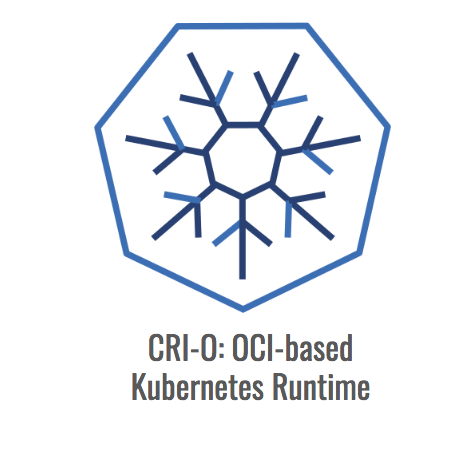
\includegraphics[width=\textwidth,height=\textwidth]{./png/crio}
%                \label{fig:guided}
%                \setcounter{subfigure}{0}% Reset subfigure counter
%        \end{subfigure}\hfill
%        }
%    \only<2-3>{
%        ~ %add desired spacing between images, e. g. ~, \quad, \qquad etc.
%          %(or a blank line to force the subfigure onto a new line)
%        \begin{subfigure}[b]{0.3\textwidth}
%        \setcounter{subfigure}{1}% Reset subfigure counter
%          \caption{Neural Network}
%                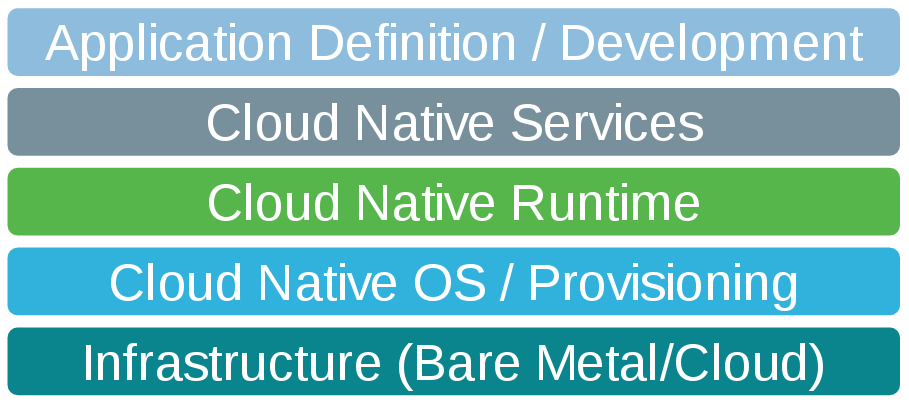
\includegraphics[width=\textwidth,height=\textwidth]{./png/cri}
%                \label{fig:free}
%        \setcounter{subfigure}{0}% Reset subfigure counter
%        \end{subfigure}\hfill
%        }
%    \only<3-3>{
%        ~ %add desired spacing between images, e. g. ~, \quad, \qquad etc.
%          %(or a blank line to force the subfigure onto a new line)
%        \begin{subfigure}[b]{0.3\textwidth}
%            \setcounter{subfigure}{2}% Reset subfigure counter
%          \caption{Matlab Output}
%                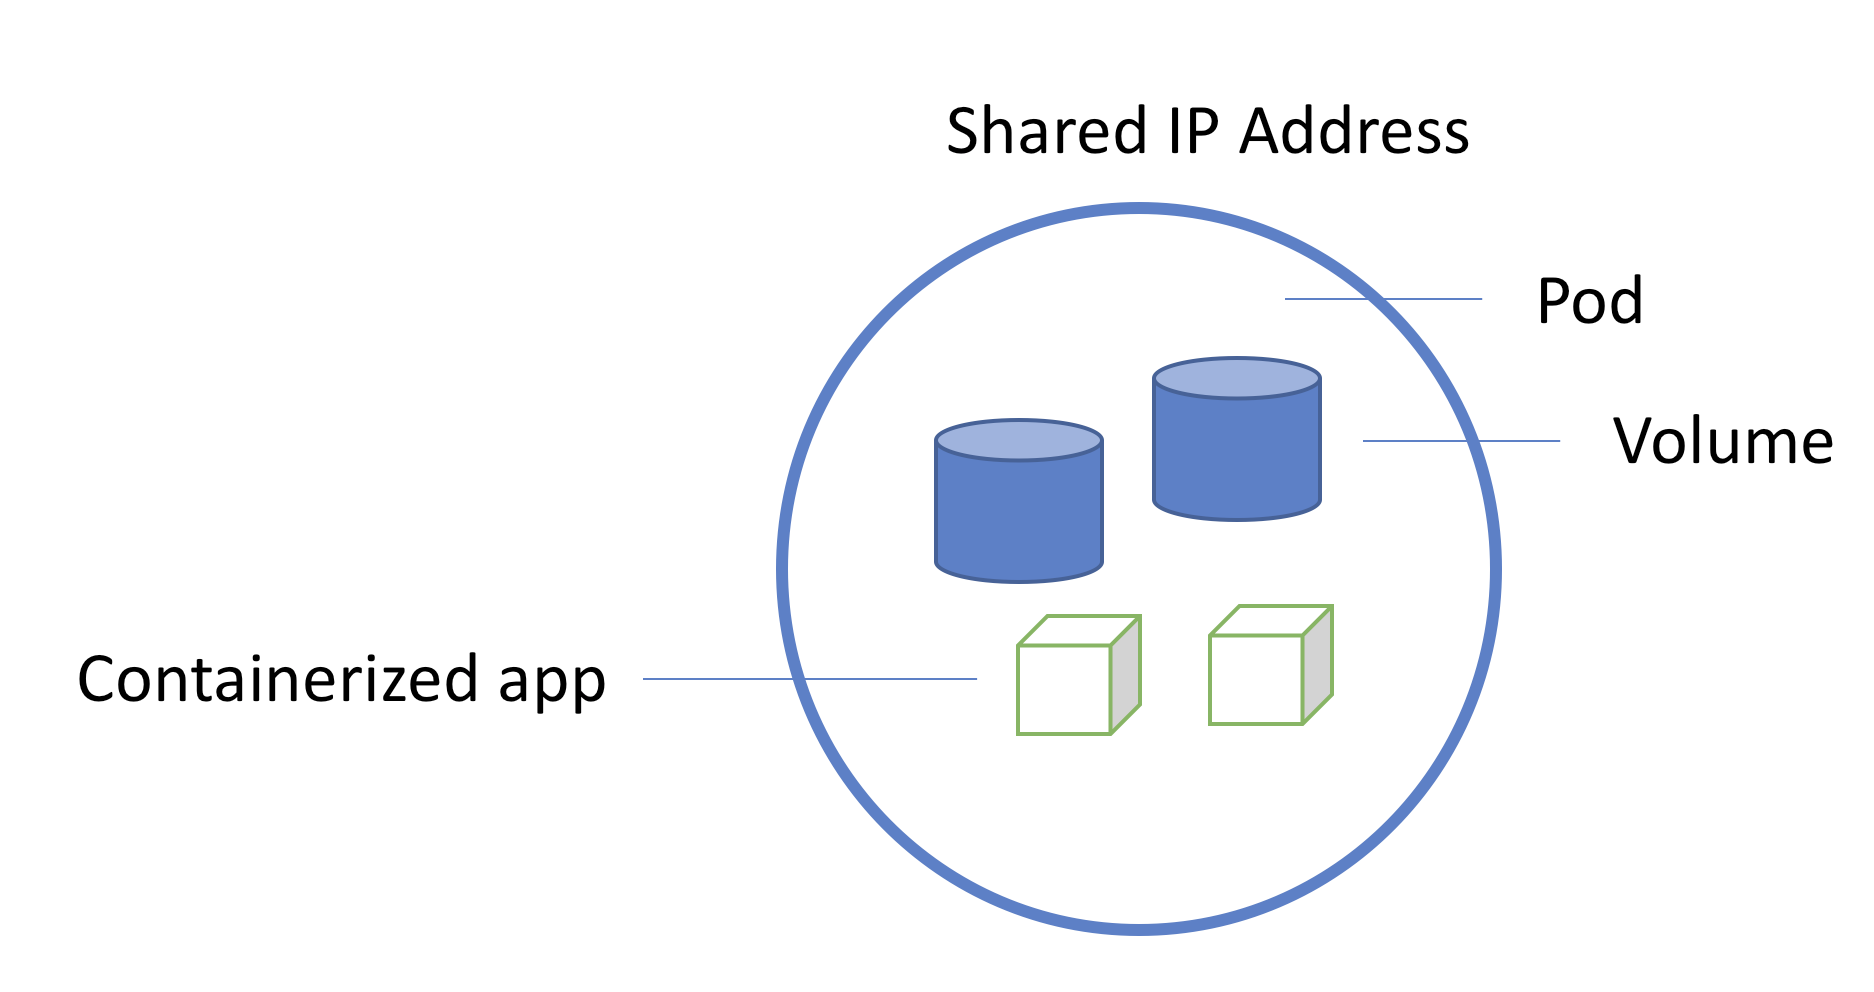
\includegraphics[width=\textwidth,height=\textwidth]{./png/pod}
%                \label{fig:multiple}
%        \end{subfigure}%
%        }
%        \caption{Different wireless charging approaches~\label{fig:animals}}
%  \end{figure}
%  \begin{itemize}[<+->]
%      \item<1-| alert@1> Free positioning charging based on Inductive coupling~\cite{wireless}.
%      \item<2-| alert@2> Based on RLoad and Frequency Input and Output~\cite{wireless}. %\ref{fig:free}
%      \item<3-| alert@3> Simulation of Matlab Output based on RLoad as an Input~\cite{wireless}. %   \ref{fig:multiple}
%  \end{itemize} 
%\end{frame}
